\chapter{Introduction to Bitcoin}
\label{sec:introbtc}

Bitcoin is a cryptocurrency and an electronic payment system built on a fully-decentralized peer-to-peer network.

It uses a \textit{permissionless} blockchain as ledger and relies on \emph{Proof-of-Work} (PoW) based probabilistic consensus algorithm to achieve eventual data consistency.

The blockchain is a public tamperproof append-only list where all the transactions are stored. The resistance to tampering comes from the blockchain structure, as shown in Section~\ref{fig:blockstruct}. Each block contains the hash of the previous one, thus makeing tampering infeasible, thus ensuring data integrity.

A Proof-of-work is a computational task given to peers, which solution is necessary to validate data appended to the blockchain. The high amount of time required to solve PoW puzzles makes attacks on the consensus algorithm infeasible, under the assumption that no user holds more than 50\% of the computing power on the network (see section~\ref{sec:securityintro}).\par

Under the assumption that no user holds more than 50\% of the computing power on the network, the PoW-based consensus algorithm achieves Byzantine fault-tolerance~\cite{nakamoto}.

While the consensus algorithm makes peers agree on the order of blocks and transactions in the ledger, the proof-of-work ensures that no adversary that owns multiple identities is capable of validating and verifying its own forged blocks.

In order to validate its own blocks the adversary would need the computational power and the time required to solve the PoW puzzle. Therefore having multiple network identities is not enough to subvert the consensus algorithm. 

Although, this implies that the result does not hold were the attacker to hold most of the computing power on the network. If that is the case, the adversary can simply keep building up its own ledger and eventually its blockchain will be authentic, generally accepted one.

In the following sections the reader will find an introduction to the Bitcoin network, where its main components and their function are analysed.


\section{An introductory example to Bitcoin usage}\label{sec:useexample}
A basic usage example, shown in Fig.~\ref{fig:basicexample}, is presented here to get the reader started with Bitcoin.

\begin{figure}[h!]
	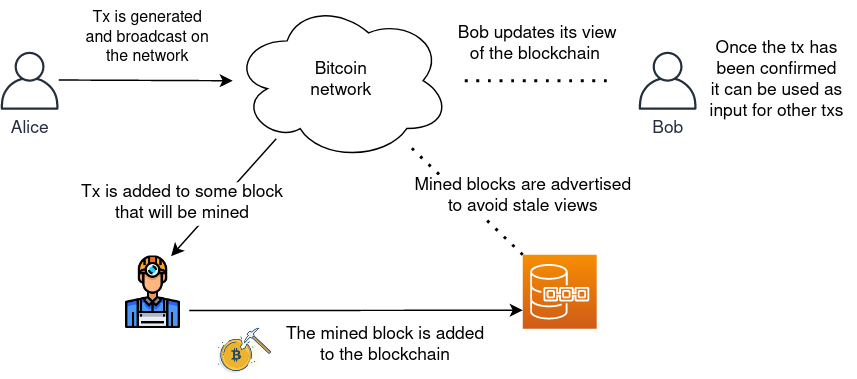
\includegraphics[width=.90\textwidth]{pict/basicexample.png}
	\centering
	\caption{Bitcoin introductory use case}
	\label{fig:basicexample}
\end{figure}

Let Alice and Bob be two Bitcoin users with a third-party wallet software. Each wallet is associated with a pair ECDSA keys used to identify users. The private key is used to sign issued transactions; instead, the public key is the Bitcoin address on which Bob can receive Bitcoins.

Suppose that Alice wants to transfer some amount of Bitcoins to Bob. Alice will generate a transaction in which she uses some set of unspent Bitcoins. The generated transaction will then be broadcast to the Bitcoin network.

A subset of the nodes, called miners, compete against one another in a parallel transaction confirmation process. Transactions are confirmed once they are included in a block added to the blockchain (\emph{mined} block).

To create a block, miners have to solve an exponentially difficult computational problem and therefore have to employ their computational power. The miner that first creates the new block earns Bitcoins, through a \emph{reward generating transaction} included in the block and the \emph{transaction fees} paid by the users whose transactions have been confirmed.

Once the transaction is included in the blockchain it is confirmed, thus the receiver will be able to spend again the transferred coins.

\section{Transaction structure}\label{sec:tx}
Transactions implement transfers and represent the entire set of coins available to users, and, when collected and ordered in the blockchain, its history. Hence, one can determine the balance of a certain wallet just by scanning the transactions on the blockchain~\cite{tschorsch-intro-survey}.

In Fig.~\ref{fig:tx} the reader can find the structure of a transaction, with its main fields.

\begin{figure}[h]
	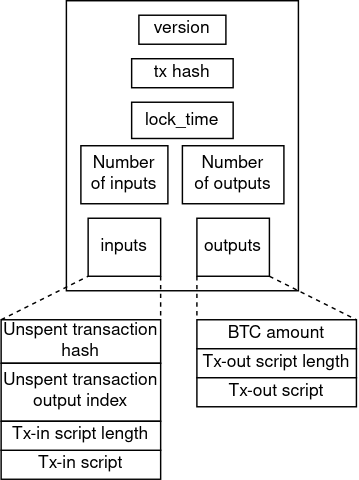
\includegraphics[width=.40\textwidth]{pict/txstruct.png}
	\centering
	\caption{Transaction structure}
	\label{fig:tx}
\end{figure}

In particular, the \texttt{lock\_time} field refers to the time or the blockchain height after which the transaction can be included in a block.

Transactions collect a set of \emph{inputs} and \emph{outputs}. Inputs are a collection of unspent coin sets, that are available to the user as previous transaction outputs or \textit{unspent transaction outputs} (UTXO). Outputs, instead, specify the number of coins to be transferred along with a receiver address.

Each input and output structure includes \emph{scripts}. These are sets of instructions, written in a Forth-like, stack-based language that describe the means to access the transferred coins. The script of a standard transaction includes a public key that, when hashed, yields a Bitcoin address, and a private key signature. The most common scripts on the market are \emph{Pay-to-PubKeyHash} (P2PKH) and \emph{Pay-to-ScriptHash} (P2SH).

Broadcasted transactions are verified before being added to a block and may be deemed invalid by honest miners and thus dropped. That might be the case for transactions that try to spend more than once the same set of coins or use invalid addresses. Nodes that broadcast invalid transactions may incur in bans if their behaviour is considered malicious.

\section{Block structure and blockchain}\label{sec:block}
The blockchain is a public distributed ledger, structured as an append-only linked list. It stores the entire transaction history of every peer in form of blocks.

In a block a set of transactions is bundled together and stored as a Merkle Tree, which ensures the data is unaltered and undamaged from the moment it is put into the block.

On top of that, each block contains the hash of the previous block in the blockchain and its own hash, thus preventing entirely block tempering for altering a transaction would result in mismatching hashes in the Merkle Tree, as well as in the stored block hash and in the hash in the next block in the blockchain.

Blocks have to be mined in order to be added to the blockchain. This means that the right \emph{nonce} needs to be found. The nonce is a varying value field that modifies the resulting hash of the block. A block is considered valid when a nonce such that the resulting hash is lower than a well-known \emph{target value} is found. That is equivalent to finding an hash that begins with $n$ zeroes.

Looking for the right nonce is exponential on $n$ number of zeroes.

The target value, and therefore the \emph{difficulty} of the computational task, is adjusted every 2016 blocks in order to keep the block generation and validation time around ten minutes.

Fig.~\ref{fig:blockstruct} shows the main fields stored in a block.

\begin{figure}[h]
	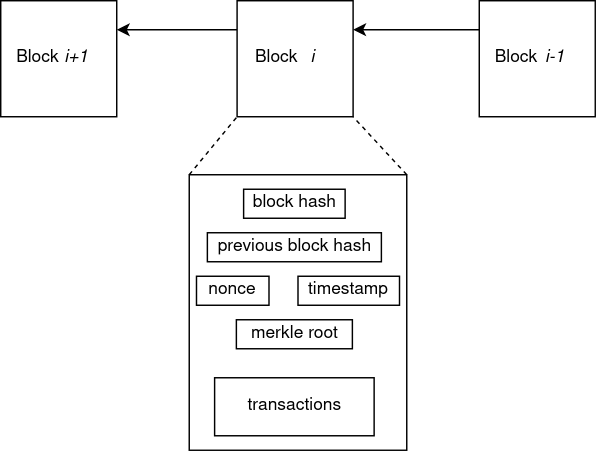
\includegraphics[width=.55\textwidth]{pict/blockstruct.png}
	\centering
	\caption{Block structure and blockchain}
	\label{fig:blockstruct}
\end{figure}

\section{Miners behaviour}\label{sec:miners}
The subset of peers that concurrently try to mine blocks by finding the right nonce are called miners, as described in Section~\ref{sec:block}. What motivates the miners to invest their computational power are mining rewards and transaction fees.

The mining reward is implemented as a transaction to the miner's wallet address that is included in the new block by the miner itself. Transaction fees are instead an amount of Bitcoins that the issuer of a transaction discretionally gives to the miners as an incentive for their work. Transactions with low transaction fees may incur in long processing times, since miners prioritize high rewards.\par

Transactions and blocks are gossiped through the network. Although each node has its own relay policy, it is in their interest, as honest miners, to get to know most of the pending transactions available for mining and to keep the view of the blockchain consistent at each node.

In particular, it is in the interest of miners to spread as fast as possible newly mined blocks in order to claim rewards and not waste time on stale views of the blockchain.

For the latter purpose, nodes need to keep their local blockchain view consistent with that of their neighbours. Nodes exchange \texttt{getblocks} messages to request \texttt{inv} messages which advertise local blocks. Missing blocks in a received \texttt{inv} message are retrieved with a \texttt{getdata} message~\cite{protocoldoc}. The described message exchange can be found in Fig.~\ref{fig:synch}.

Furthermore, \texttt{inv} messages are also gossiped when a node receives a new block. It is relevant to note that new blocks will be dropped by the receiving peers if any transaction is invalid or already spent. Nodes implicitly accept a block by starting to work on the next one, which contains the hash of last received valid block. 

\begin{figure}[h]
	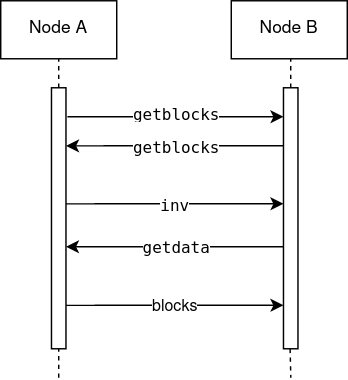
\includegraphics[width=.35\textwidth]{pict/blockchain-synch.png}
	\centering
	\caption{blockchain synch}
	\label{fig:synch}
\end{figure}

\section{Proof-of-Work and Consensus protocol}\label{sec:consensus}
In Bitcoin, as well as in other cryptocurrencies, the transaction verification process (mining) is distributed. The legitimacy of a transaction is verified by the majority of nodes before it is added to the public ledger, the blockchain.

These distributed environments are vulnerable to attacks in which a malicious user connects multiple fake replicas of himself to the network. If the number of fake attacking nodes exceeds that of the honest nodes, the attacker can forge any kind of data and validate it, thus appending it to the blockchain.

To avoid such scenarios, in order to append data to the blockchain, a Proof-of-Work is required. PoWs are cryptographic math puzzles that require scanning for a value, the nonce, which correct value attests that the node has put computational effort and time to verify the transaction(s). Mining is also described in Section~\ref{sec:useexample} and~\ref{sec:block}.

Thus, PoW discourages any kind of data forgery. Furthermore, tempering on the blockchain is impossible thanks to the definition of Merkle tree and blockchain, as described in Section~\ref{sec:block}. Bitcoin is therefore resistant both to tempering and forgery.

As mining is defined as a distributed process, and due to the lack of any central ledger, nodes may share inconsistent views of the blockchain. This is the case if relayed blocks are not delivered to some nodes or two or more nodes mine a new block approximately at the same time.

\emph{Forks} on the blockchain that are not maliciously engineered are solved by themselves by following a simple rule: only the longest branch of the blockchain is considered valid.

If two nodes are working on different branches of the same height, due to the random nature of mining, eventually one will release a new block before another. Hence its blockchain will be the longest and the only one considered correct.

To ensure that all nodes agree on the order of the entries of the blockchain, some simple rules are defined. More specifically, they state that:
\begin{enumerate}
	\item input and output values are rational
	\item transactions only spend unspent outputs
	\item all inputs being spent have valid signatures
	\item no transactions spend inputs with a \texttt{time\_lock} before the block in which they are confirmed
\end{enumerate} 
 
Bitcoin's PoW-based distributed consensus algorithm is defined as probabilistic since it guarantees eventual consistency. Furthermore it is generally considered robust and extremely scalable, as no authorization is required to join the network and mine.\par